\section{Physikalische Grundlagen \label{Grundlagen}}

\begin{figure}[h!]
    \centering
    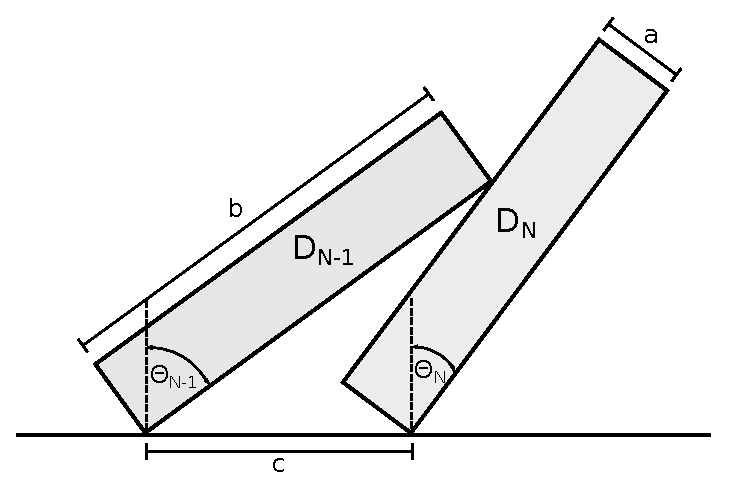
\includegraphics[width=.7\linewidth]{schema}
    \caption{Schema}
    \label{abb:1}
\end{figure}

\noindent
Wir betrachten zunächst zwei aufeinanderfolgende Dominosteine wie in
(\ref{abb:1}). Geht man davon aus, dass die Dominos nur rotieren können und
daher nicht von ihrem Auflagepunkt abweichen, können wir die folgende
trigonometrische Beziehung ableiten:

\begin{equation}
    \sin(\Theta_{N-1} - \Theta_{N}) = \frac{c}{b} \cos(\Theta_{N}) - \frac{a}{b}
    \label{eq:1}
\end{equation}

\noindent
Die zeitliche Ableitung liefert schließlich:

\begin{equation}
    \dot{\Theta}_{N-1} = \left[
        1-\frac{c}{b}
        \frac{\sin{\Theta_{N}}}
        {\cos{\left(\Theta_{N-1}-\Theta_{N}\right)}}
    \right]
    \label{eq:2}
\end{equation}

Das Zeitintervall $t_N$ beschreibt die Zeit, in der ein Dominostein $D_N$ sich
aus seiner vertikalen Position herausbewegt bis er schließlich Kontakt zum
Domino $D_N$ hat. Wir erhalten genau diese Zeit durch die Energiebetrachtung.
Die Gesamtenergie $E$ des Systems setzt sich zusammen aus der kinetischen und
potentiellen Energie von allen Dominos in Bewegung.
Prinzipiell erhalten wir mit den Anfangsbedingungen bereits an dieser Stelle
eine Gleichung für $\Theta_N$. Eine analytische Lösung der Rekursionsformel ist
aufgrund der gegebenen Komplexität jedoch nicht möglich und wir entwickeln
einen numerischen Ansatz:

\begin{equation}
    \begin{split}
        \cos{\Theta_i} & = U_i\cos{\Theta_N} \nonumber \\
        \sin{\Theta_i} & = V_i\sin{\Theta_N} \label{eq:3} \\
        \dot{\Theta}_i & = W_i\dot{\Theta}_N \nonumber
    \end{split}
\end{equation}

Die Koeffizienten $U_i$, $V_i$, $W_i$ werden durch wiederholte Anwendung der
Rekursionsformel (\ref{eq:1}) und (\ref{eq:2}) gewonnen. Aus (\ref{eq:3})
erhalten wir eine Gleichung für $\dot{\Theta}_N$.

\begin{equation}
    \dot{\Theta}_N = \sqrt{\frac{2E - mg
        \left( b\cos{\Theta_N} \sum_{i=1}^N U_i
        + a\sin{\Theta_N} \sum_{i=1}^N V_i \right)}
    {I \sum_{i=1}^N W_i}}
    \label{eq:4}
\end{equation}

\noindent
Die Zeit $t_N$ erhalten wir nun durch einfache Integration:

\begin{equation}
    t_N = \int_0^{\Theta_C} \frac{1}{\dot{\Theta}_N} \mathrm{d}\Theta_N
    \label{eq:5}
\end{equation}

Wobei $\Theta_C$ denjenigen Winkel darstellt, bei dem ein Domino gerade mit der
oberen Kante Kontakt zum nächsten Domino hat.

Zuletzt betrachten wir die Drehimpulserhaltung in Anhängigkeit von
$\dot{\Theta}_N'$ sowie $\dot{\Theta_N''}$. Erstere Größe beschreibt die
Winkelgeschwindigkeit kurz nach dem Kontakt von $D_N$ mit $D_{N+1}$, letztere
die Geschwindikeit davor.

\begin{equation}
    I \displaystyle\sum_{i=1}^N \dot{\Theta}_N'' =
    I \displaystyle\sum_{i=1}^{N+1} \dot{\Theta}_N'
    \label{eq:6}
\end{equation}

Zusammen mit der obigen Annahme für einen numerischen Lösungsansatz erhalten
wir:

\begin{equation}
    \dot{\Theta}_{N+1}' =
        \frac{\sum_{i=1}^{N} W_i''}{\sum_{i=1}^{N+1} W_i'}
        \dot{\Theta}_N''
    \label{eq:7}
\end{equation}

$W_i''$ und $W_i'$ beschreiben $W_i$ vor bzw. nach dem Kontakt.

Insgesamt können wir mithilfe von Gleichung (\ref{eq:7}) sowie $\dot{\Theta}_i
= W_i\dot{\Theta}_N$ zu allen Dominos die jeweilige Anfangswinkelgeschwindikeit
angeben. Diese Wert dienen der Berechnung der Energie $E$, welche für das
nächste Intervall $t_{N+1}$ relevant ist.
Die Gesamtzeit, welche die Kette benötigt um komplett zu fallen, erhalten wir
schließlich aus der Summation von allen Intervallen $t_i$.

Am Ende des Projektes soll eine Simulation mit genau diesem physikalischen
Hintergrund durchgeführt worden sein.
